Partiendo de la arquitectura base descrita en los capítulos anteriores, en esta sección se analizan las mejoras exploradas para incrementar la eficacia del sistema multiagente.

Para ello, se han integrado tres mecanismos complementarios: un prompting con ejemplos ilustrativos (\textit{few-shot}), un sistema de memoria persistente y un diseño adaptativo que modifica el comportamiento del sistema según la complejidad de la consulta formulada.

\section{Prompting Few Shot}
El aprendizaje mediante ejemplos de entrada consiste en proveer al LLM ejemplos del comportamiento esperado para ajustar la salida de este, obteniendo mejoras de rendimiento para tareas específicas de forma flexible, únicamente modificando el prompt de entrada \cite{brown_language_2020}.

El comportamiento del orquestador y planificador son perfectos para esta estrategia, ya que hay varios escenarios generales donde se quiere que actúen de cierta forma. Por ejemplo, se requiere que el agente planificador ajuste su plan dinámicamente en función de la información recavada. El Listado \ref{lst:few_shot} ilustra un ejemplo donde se le instruye al agente que tiene la capacidad de razonar si finalizar el plan, aún en contra de lo planeado inicialmente. Se le indica el contexto en el que se encuentra, la respuesta esperada y una explicación del comportamiento esperado. 

\begin{lstlisting}[caption={Integración de ejemplos few shot al agente planificador},label={lst:few_shot}]
  examples = [
      {
          "current_info": "The previous plan was to find information about X and then about Y. Information about X was gathered",
          "question": "Provide information about X and Y",
          "plan": "Enough information for X and Y was gathered. Finished",
          "explanation": "Dynamically adjust your plan as you go, some steps might be unnecessary"

      },
      ...
  ]

  # Indicar la plantilla con la que se convertirá cada ejemplo en el prompt
  example_prompt = PromptTemplate.from_template("\t{explanation}:\n\t\tCurrent information:{current_info}\n\t\tQuestion:{question}\n\t\tPlan:{plan}")

  # Aplicar la plantilla a todos los ejemplos
  def get_planner_few_shots(examples_list: List[dict]):
      few_shots_template = FewShotPromptTemplate(
          examples=examples_list,
          example_prompt=example_prompt,
          input_variables=[],
          suffix="",
          prefix="Here are some abstract examples:"
      )
      return few_shots_template.format()
  planner_few_shots = get_planner_few_shots(examples)
\end{lstlisting}

Los ejemplos se han redactado de forma abstracta respecto al proyecto software utilizado. No se ha incluído información del comportamiento esperado respecto a fuentes de datos o agentes específicos, para evitar el sobreajuste de este respecto a los datos anotados. 

\section{Memoria persistente}
La memoria persistente constituye en proveer al agente información de ejecuciones anteriores para ampliar su conocimiento, simulando funciones cognitivas humanas (Véase Sección \ref{sec:modulos_memoria}). 

Este enfoque se ha implementado en los agentes especializados, con el objetivo de mejorar la búsqueda de información. De esta forma, el agente obtendrá resúmenes de respuestas anteriores que sean relevantes para la consulta actual, proporcionando información complementaria que el agente podría no haber extraído correctamente. 

La Figura \ref{fig:mem_1} ilustra el funcionamiento de dicho mecanismo. En primer lugar, se añaden al prompt del agente memorias relevantes realizando una búsqueda RAG sobre un objeto \opus{AsyncPostgresSaver}. Este representa una abstarcción de LangChain para guardar elementos en PostgreSQL, similar a \opus{PGVector} utilizado en la Sección \ref{sec:agente_filesystem}. Una vez el agente ha generado su respuesta, un agente resumidor comprime el resultado en aproximadamente 75 carácteres. Este resumen se indexa en la base de datos utilizando dicha abstracción, guardando adicionalmente las citas referenciadas.

\begin{figure}[h]
\centering
\adjustbox{center=\textwidth}{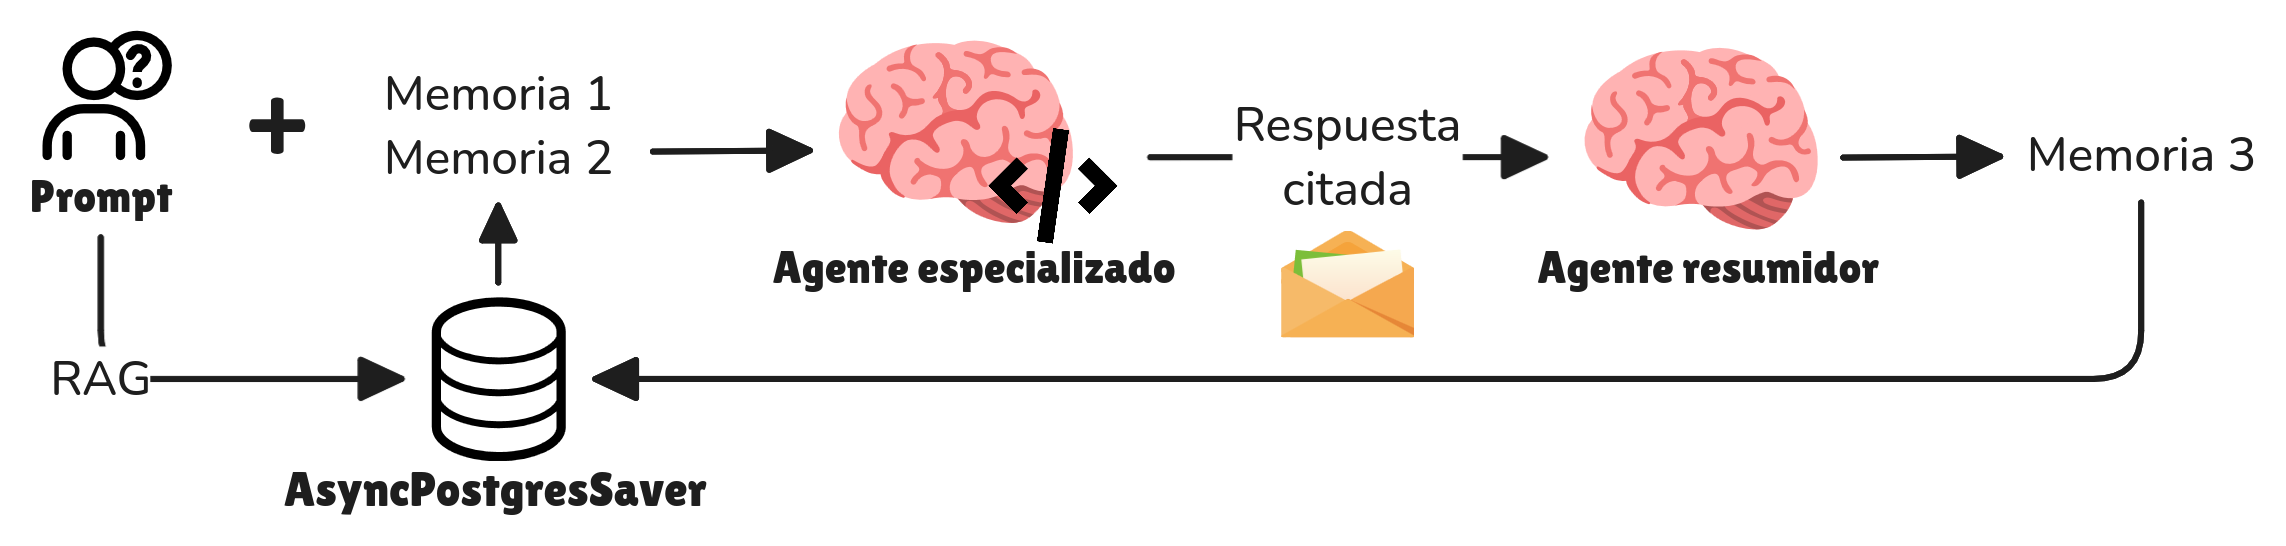
\includegraphics[width=1\linewidth]{figures/memoria_1.png}}
\caption{Flujo operativo del sistema de memoria de los agentes especializados}
\label{fig:mem_1}
\end{figure}

La extracción de las memorias se realiza mediante un RAG híbrido. En lugar de obtener únicamente las memorias más parecidas al prompt actual, se considera también las veces que estas han sido accedidas, favoreciendo las memorias que más veces han sido accedidas. De este modo, se calcula la relevancia final teniendo en cuenta en un 75\% la puntuación de relevancia y en un 25\% la puntuación de acceso. Esta última se obtiene en relación a la memoria más accedida. Por ejemplo, si la memoria más accedida se ha extraído 10 veces, y la memoria actual ha sido accedida 5 veces, la puntuación para ello será de 0.5. Si la puntuación de relevancia semántica es a su vez 0.8, la media ponderada será de 0.725.

\subsection{Agrupación de memoria}
Para evitar que conceptos relevantes se pierdan ante un conjunto de memorias excesivamente grande, se ha implementado un sistema de agrupación que resume pasajes parecidos en memorias unificadas, replicando el olvido de la memoria humana. 

La Figura \ref{fig:mem_2} ilustra dicho sistema. Cuando las memorias de un agente especializado específico llegan a cierto número, se ejecuta el sistema de agrupación. Este ejecuta primero una agrupación semántica de las diferentes memorias en los denominados \textit{clusters}. Para ello se utiliza el algoritmo KMeans Clustering, de la librería scikit-learn\footnote{scikit-learn: \url{https://scikit-learn.org/stable/}}. Este algoritmo agrupa las diferentes memorias basándose en la distancia entre las diferentes dimensiones de los embeddings, siendo dos memorias más parecidos semánticamente en caso de tener embeddings más cercanos. 

\begin{figure}[h]
\centering
\adjustbox{center=\textwidth}{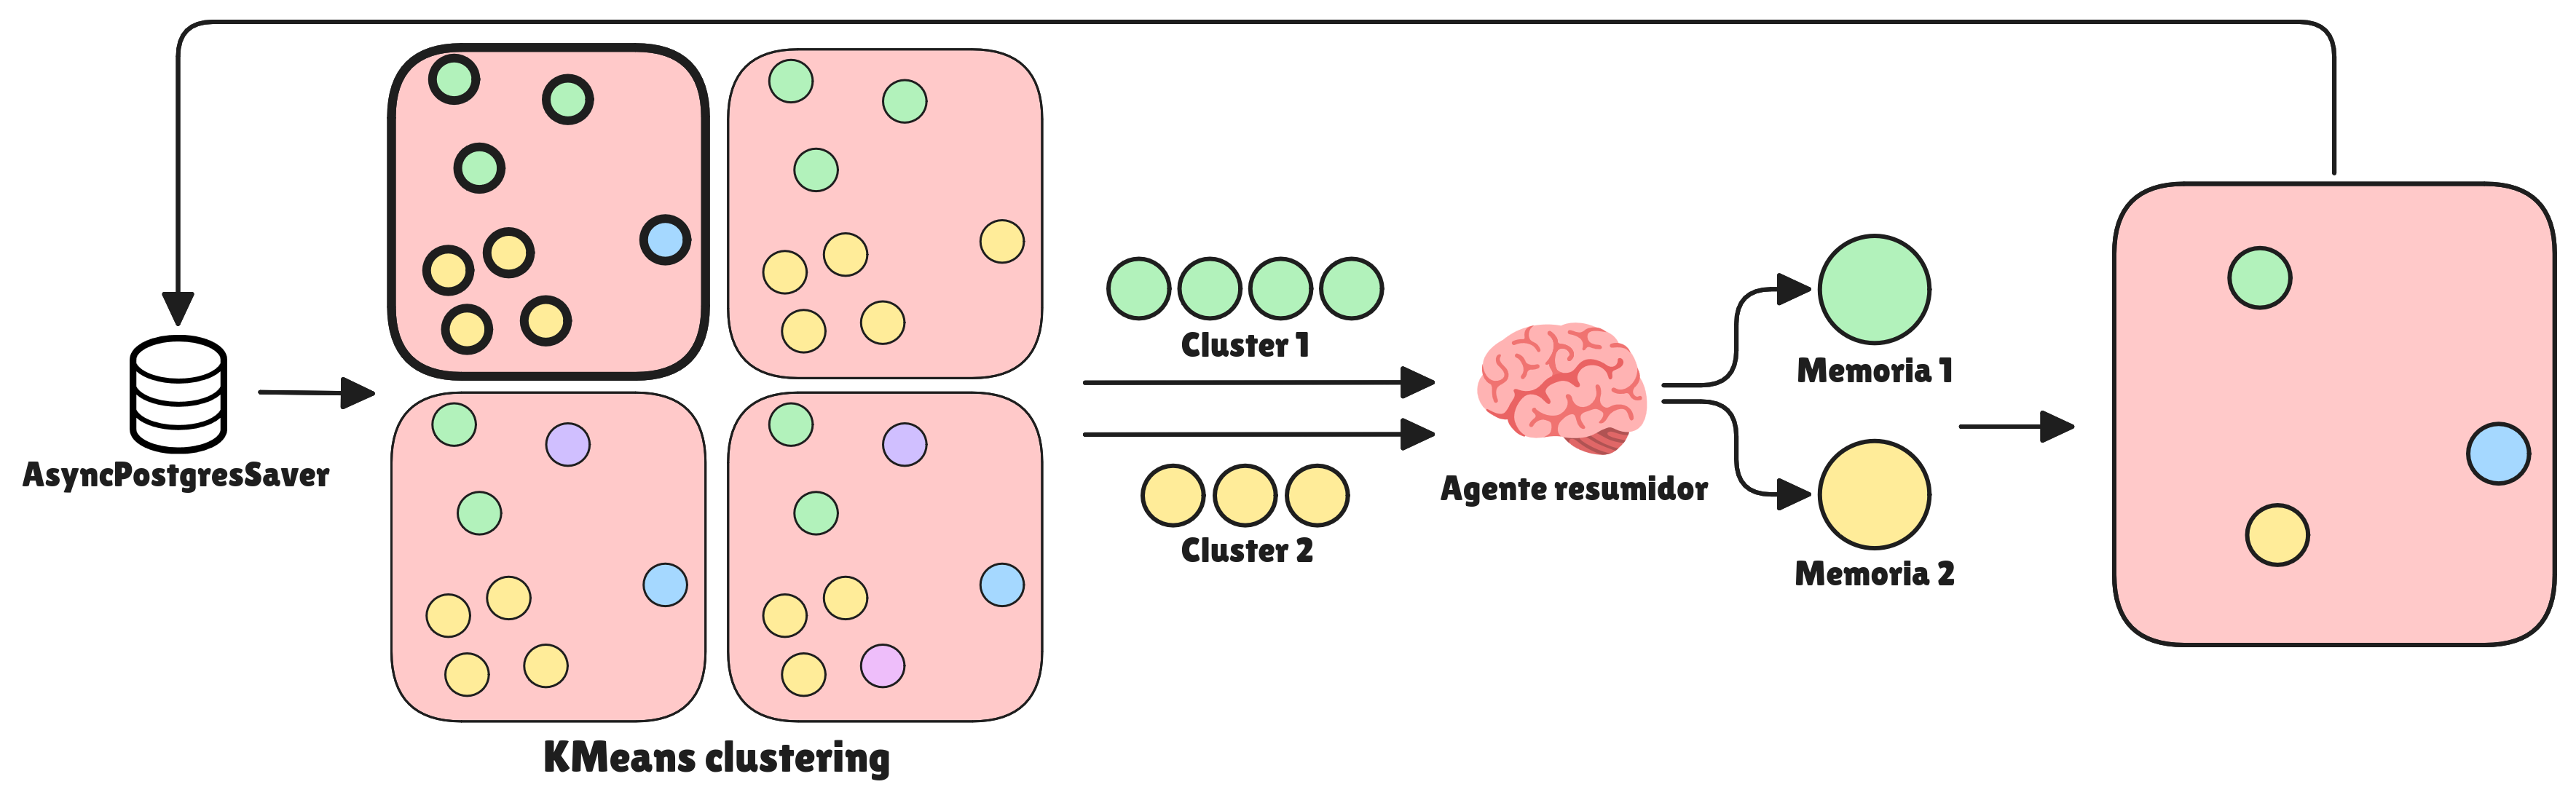
\includegraphics[width=1.25\linewidth]{figures/memoria_2.png}}
\caption{Agrupación de memoria por clusters}
\label{fig:mem_2}
\end{figure}

Una vez distinguidos los diferentes clusters, un agente resumidor agrupa todas las memorias de cada cluster en memorias individuales. Al ser estos parecidos semánticamnete, este debería ser capaz de abstraer los conceptos comunes en todas las memorias a otra memoria. Estas memorias agrupadas se añaden a la base de datos, eliminando a su vez las memorias originales del cluster. 

Para determinar el número óptimo de clusters, se ha aplicado el método del codo. Esta técnica calcula la suma de distancias entre cada elemento y el centro de su cluster para distintas cantidades de grupos. A medida que aumenta el número de clusters, la distancia total disminuye (ya que al haber menos elementos por grupo, cada uno está más cerca de su centro); sin embargo, el punto de mayor inclinación (calculado mediante la segunda derivada) representa el equilibrio óptimo. La Figura \ref{fig:codo} muestra los resultados de este análisis, identificando 3 como el número ideal de clusters.

La Figura \ref{fig:clustering-analysis} ilustra el agrupamiento de 12 memorias del agente de código en los mencionados 3 clusters, mientras que la Figura \ref{fig:clusters} presenta la simplificación de sus embeddings a un espacio bidimensional. En esta última visualización se observan los tres grupos identificados, confirmando la diferenciación  .

\begin{figure}[htbp]
    \centering
    \subfloat[Visualización de clusters en dos dimensiones\label{fig:clusters}]{
        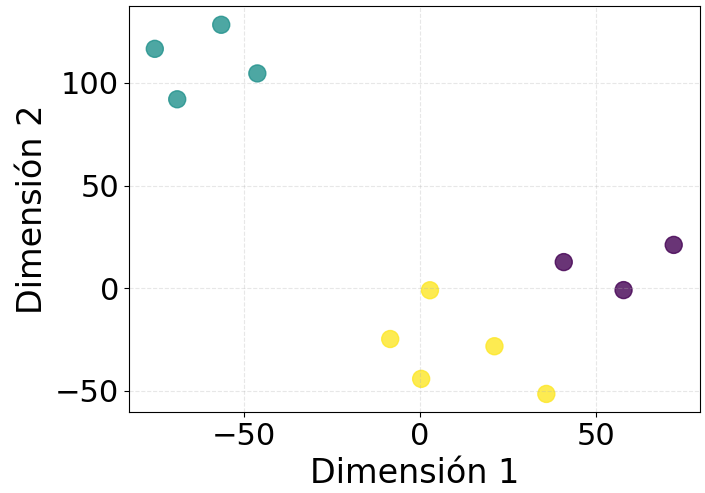
\includegraphics[width=0.40\textwidth]{figures/cluster_2.png}
    }
    \subfloat[Método del codo sobre agrupación de clusters\label{fig:codo}]{
        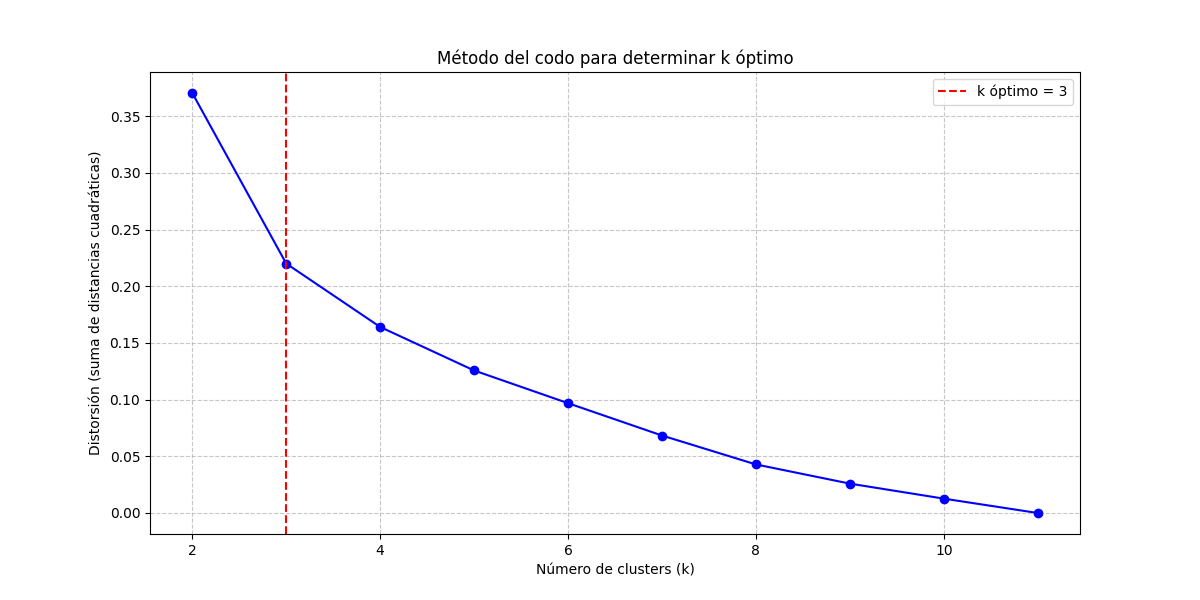
\includegraphics[width=0.65\textwidth]{figures/codo.png}
    }
    \caption{Agrupación de 3 clústeres}
    \label{fig:clustering-analysis}
\end{figure}

\section{Diseño adaptativo}
Tras evaluar los enfoques expuestos en el capítulo anterior (Véase Sección \colorbox{yellow}{\ref{}}), los resultados muestran que aunque con un rendimiento superior, el paso de planificación añade una complejidad considerable frente al enfoque más simple. Mientras que el sistema simple es capaz de responder algunas preguntas con mayor rapidez, no consigue resolver las preguntas más difíciles. Es por ello que un sistema híbrido surge como la solución ideal \cite{}, utilizando la planificación para preguntas complejas y omitiéndolo cuando no es necesario.

La implementación de este enfoque se ha estructurado en tres fases: la determinación de criterios para identificar preguntas complejas, la ampliación del conjunto de evaluación para mejorar la precisión de evaluación, y el análisis comparativo entre un modelo especializado y un agente clasificador. Finalmente, se procedió a la integración del clasificador seleccionado en el flujo del sistema.

\subsection{Criterios de clasificación}
Para determinar qué tipos de preguntas clasificar como difíciles, se han empleado las evaluaciones detalladas en la Sección \colorbox{yellow}{\ref{}}. Se consideran difíciles aquellas preguntas en las que se cumple cualquiera de estas condiciones: el resultado de evaluación es peor en la orquestación simple que en la compleja, o el resultado de evaluación es menor a 0.5 en cualquiera de las dos orquestaciones. Esto resultó en un total de 19 preguntas difíciles y 27 fáciles. 

Tras analizar ambos conjuntos, quedó claro que las consultas que más desafían al sistema son aquellas cuyas fuentes de información no son triviales de acceder. Por ejemplo, el sistema no tiene problemas en responder preguntas genéricas de gestión, ya que determinar cuál agente contiene dicha información es sencillo. Por el contrario información, sobre módulos o implementaciones específicas es más difícil de ubicar: \texttt{¿Dónde puedo encontrar la documentación técnica actualizada para las tecnologías o herramientas específicas?}. La ubicación de esta información no es clara, podría estar en la documentación general, en Confluence, o incluso en el repositorio de código. 

\subsection{Aumento de datos}
Tras determinar los criterios de clasificación, se instruyó al modelo Calude Sonnet con dichos criterios y el contexto del proyecto, aumentando las preguntas originales a 200 ejemplos únicos.

Tras esto, se utilizó la técnica de aumento sencillo de datos (EDA) \cite{} sobre dichos ejemplos. Esto consiste en realizar una serie de operaciones sobre los ejemplos originales para variar ligeramentesu composición, reemplazando palabras por sinónimos, alterando el órden de algunas palabras, u omitiendo palabras específicas. Para ello se ha utilizado el script\footnote{\url{https://github.com/jasonwei20/eda_nlp}} desarrollado por los autores de dicha técnica, obteniendo un total de 2000 preguntas tras el aumento.   
Estos ejemplos se dividieron en tres conjuntos individuales: entrenamiento (75\%), evaluación (15\%) y pruebas (15\%). Todas las preguntas resultantes de la técnica EDA para una sola pregunta original deben de estar en el mismo conjunto, ya que al ser muy parecidas sesgarían los resultados de evaluación. Finalmente se subieron a un dataset público en HuggingFace\footnote{Dataset de preguntas: \url{https://huggingface.co/datasets/MartinElMolon/tfg_clasificador}}. 

\subsection{Clasificación de preguntas}
Para clasificar las consultas del usuario por dificultad, se han utilizado dos enfoques alternativos: 

\begin{itemize}
  \item\textbf{Agente clasificador: }Añadiendo en el prompt tanto los criterios de clasificación, tanto 5 ejemplos representativos de cada clase, el agente debe determinar mediante una salida estructurada la dificultad de la pregunta.
  \item\textbf{Modelo clasificador: }Se ha utilizado el modelo especializado en clasificación RoBERTa-base\cite{}, en su versión entrenada con un corpus textual derivado de la biblioteca nacional de españa\cite{}. Dicho modelo se ha ajustado con el dataset mencionado en la sección anterior. Los detalles del entrenamiento están disponibles en el anexo \ref{}, mientras que el modelo está públicamente disponible en HuggingFace\footnote{Modelo: \url{https://huggingface.co/MartinElMolon/RoBERTa_question_difficulty_classifier}}.
\todo{Omitir los detalles de entrenamiento en la memoria principal y añadirlos en el anexo es una buena idea? Así evito explicar conceptos que no tienen que ver con la ingeniería del software y es todo más simple.

También podría no ponerlos directamente}
\end{itemize}

\subsubsection{Evaluación de ambos enfoques}
Ambos modelos se han evaluado con el conjunto de prueba de 300 preguntas, siendo el agente clasificador usando el modelo gpt4.1-mini ligeramente superior en un 3\% (91\% frente a 88\%).

Dichos resultados muestran el potencial de integrar modelos especializados en flujos agénticos. El LLM ajustado obtiene un rendimiento similar con aproximadamente 2 órdenes de magnitud menos de complejidad, teniendo este 125 millones de parámetros frente a las decenas de miles de millones de modelos comparables al gpt propietario utilizado. Adicionalmente, este se ha ejecutado en la CPU local, obteniendo un tiempo de respuesta inferior. 

Cabe destacar que el enfoque con el modelo reducido presenta una serie de inconvenientes que lo hacen viable únicamente en escenarios concretos. Al depender este de un entrenamiento previo, su modificación es menos flexible. Mientras que para modificar el comportamiento del LLM grande basta con modificar el prompt, el LLM pequeño requeriría de un reentrenamiento, con un conjunto de datos modificado que representen los cambios a introducir. 




